\section{Theorie}
\label{sec:Theorie}
Unter dem Faraday-Effekt versteht man die Drehung der Polarisationsebene einer elektromagnetischen Welle in einem Medium durch den Einfluss eines Magnetfeldes, welches parallel zur Ausbreitungsrichtung dieser ist. \\
Außerdem ist es möglich Rückschlüsse auf die Bandstruktur des Testmediums zu ziehen.
\subsection{Elektronische Struktur von Isolatoren, Halbleitern und Metallen}
\label{sec:Isolatoren}
Wie in Abschnitt \ref{sec:Isolatoren} erwähnt
In Abbildung \ref{fig:leiter} sind die jeweiligen Bandstrukturen von Isolatoren (Nichtleitern), Halbleitern und Metallen (Leitern) dargestellt:
\begin{figure}
  \centering
  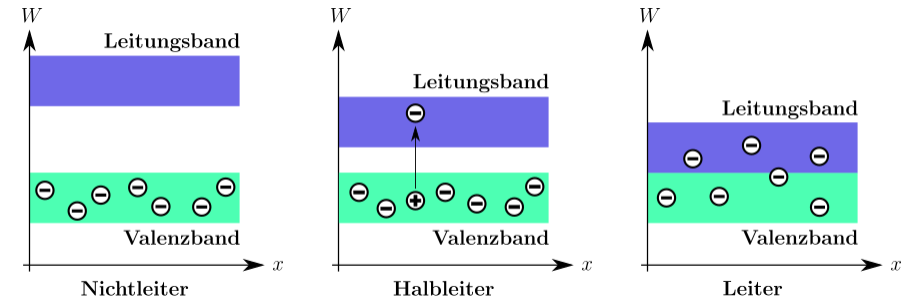
\includegraphics[scale=0.45]{fig/leiter.png}
  \caption{Bandstruktur von Isolator, Halbleiter und Metall. \cite{Bild5}}
  \label{fig:leiter}
\end{figure}
\subsubsection{Isolator}
Wie in Abbildung \ref{fig:leiter} zu sehen ist, ist das Leitungsband eines Isolators unbesetzt und die Bandlücke ist sehr groß. Dennoch kann durch Zufuhr von großer Energie es möglich sein, dass Elektronen die Bandlücke überwinden können und vom Valenzband ins Leitungsband gelangen können. Isolatoren zeichnen sich also über einen sehr hohen spezifischen Widerstand aus, der jedoch nicht unendlich ist, das heißt sie können auch leitend werden.
\subsubsection{Halbleiter}
Ähnlich wie bei den Isolatoren besitzen Halbleiter ein unbesetztes Leitungsband (siehe Abbildung \ref{fig:leiter}), allerdings ist die Bandlücke deutlich kleiner als bei Isolatoren und Elektronen können diese leicht überwinden. Mit Hilfe von Dotierung, das bedeutet das Entfernen oder Hinzufügen eines Fremdatoms, kann der Halbleiter gezielt manipuliert werden. Unter n-Dotierung versteht man hierbei wenn ein sogenannter Elektronen-Donator, das heißt ein Atom mit zusätzlichem Elektron, in den Halbleiter eingebunden wird. Unter p-Dotierung das Gegenteil, das heißt ein Elektronen-Akzeptor, ein Atom mit mit einem Elektron weniger, wird in den Halbleiter eingebunden.
\subsubsection{Metall}
In Abbildung \ref{fig:leiter} erkennt man, dass es bei Metallen keine Bandlücke gibt. Daraus folgt, dass in Metallen Elektronen sich schon bei sehr geringen elektrischen Feldstärken nahezu frei bewegen können. Dies bedeutet, dass ein Metall ein sehr guter
elektrischer Leiter ist. Zu beachten ist, dass die durch den Stromfluss induzierte Temperaturerhöhung im Metall den Widerstand erhöht und somit das Metall einen temperaturabhängigen Widerstand besitzt.
\subsection{Definition der effektiven Masse}
\label{sec:effektive_masse}
Mit Hilfe der effektiven Masse ist es möglich die physikalischen Effekte der Bandstruktur eines Halbleiters approximiert zu beschreiben. In Abbildung \ref{fig:band} ist die Bandstruktur von Leitungs- bzw. Valenzband dargestellt.
\begin{figure}
  \centering
  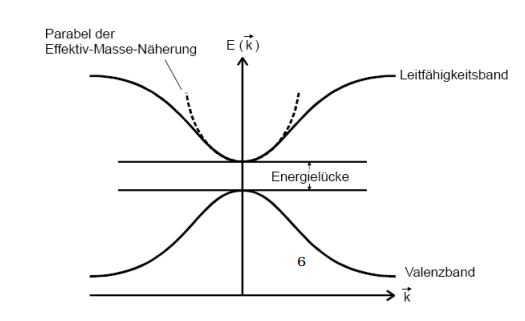
\includegraphics[scale=0.7]{fig/band.png}
  \caption{Vereinfachte Darstellung der Bandstruktur eines Festkörpers. \cite[6]{Bild2}}
  \label{fig:band}
\end{figure}
Um das Minimum herum wird die Energie des Bandes $\varepsilon$ in Abhängigkeit des Wellenzahlvektors $\vec{k}$ genähert. Dies geschieht mit Hilfe einer Taylorreihe:
\begin{equation}
  \label{eqn:energiegl}
  \varepsilon(\vec{k})=\varepsilon(0) + \frac{1}{2}\sum_{i=1}^3 \left.\frac{\partial^2 \varepsilon}{\partial k_i^2}\right|_{k=0}k_i^2 + \mathcal{O}(k^3)
\end{equation}
Als nächstes vergleicht man analog zu Newtons zweitem Axiom die Beschleunigung in einem elektrischen Feld $E$. Dafür ergibt sich quantemechanisch betrachtet für ein Kristall-Elektron (\ref{eqn:kris})
 und für ein freies Teilchen im Vakuum (\ref{eqn:frei}):
\begin{align}
  \label{eqn:kris}
  a&=\dfrac{1}{\hbar^2}\dfrac{\partial^2 \varepsilon}{\partial k^2}\cdot qE \\
  \label{eqn:frei}
  a&=\dfrac{1}{m_e}\cdot qE
\end{align}
Dabei ist $k$ die Wellenzahl, $\hbar$ das reduzierte plancksche Wirkungsquantum, $q$ die Ladung des Elektrons und $\varepsilon(k)$ die Energie in Abhängigkeit von $k$.
Damit wird die effektive Masse wie folgt definiert:
\begin{equation}
  \label{eqn:effmass}
  m^{*}_i := \frac{\hbar^2}{\left.\frac{\partial^2 \varepsilon}{\partial k_\mathrm{i^2}}\right|_\mathrm{k=0}}
\end{equation}
Dank der Berücksichtigung der Periodizität des Kristallpotentials $V(\vec{r})$ in dem Ausdruck für die effektive Masse siehe Gleichung (\ref{eqn:effmass}) ist es unter Anderem möglich den Hamilton-Operator $\hat{H}$ der Kristallelektronen in den
eines freien Teilchens umzuschreiben. Aus
\begin{equation*}
  \hat{H}=\dfrac{\hbar^2}{2m_\mathrm{e}}\nabla^2+V(\vec{r})
\end{equation*}
wird mit Gleichung (\ref{eqn:effmass})
\begin{equation*}
  \hat{H}=\dfrac{\hbar^2}{2m^*}\nabla^2 .
\end{equation*}
\subsection{Zirkulare Doppelbrechung}
\label{sec:zirkulare_doppelbrechung}
In diesem Abschnitt der Theorie geht es um zirkulare Doppelbrechung. Darunter versteht man die Drehung der Polarisationsebene von linear polarisiertem Licht $E(z)$ bei Transmission durch einen Kristall.
Dies lässt sich durch die unterschiedlichen Phasengeschwindigkeiten im Kristall für rechts- bzw. linkszirkulares polarisiertes Licht $E_\mathrm{R}$, $E_\mathrm{L}$ erklären. Mathematisch bedeutet das für
die Zusammensetzung des Lichtstrahls als Linearkombination von $E_\mathrm{R}$ und $E_\mathrm{L}$:
\begin{equation}
  \label{eqn:zusammen}
  \vec{E}(z)=\dfrac{1}{2}(\vec{E}_\mathrm{R}(z)+\vec{E}_\mathrm{L}(z)) \, \mathrm{mit} \, k_\mathrm{L}\neq k_\mathrm{R}
\end{equation}
Die rechts- bzw. linkszirkularen Anteile sind wie folgt definiert:
\begin{align}
  \label{eqn:rechtslinks}
  \begin{aligned}
  \vec{E}_\mathrm{R}(z) &= \left(E_\mathrm{0} \vec{x}_\mathrm{0} - \mathrm{i}E_\mathrm{0}\vec{y}_\mathrm{0}\right)\exp\left(\mathrm{i}{k}_\mathrm{R}z\right)\\
  \vec{E}_\mathrm{L}(z) &= \left(E_\mathrm{0} \vec{x}_\mathrm{0} + \mathrm{i}E_\mathrm{0}\vec{y}_\mathrm{0}\right)\exp\left(\mathrm{i}{k}_\mathrm{L}z\right).
\end{aligned}
\end{align}
Um nun das austretende Licht zu beschreiben werden zunächst zwei Winkel $\Psi$ und $\vartheta$ eingeführt:
\begin{align}
  \label{eqn:winkel}
  \begin{aligned}
    \Psi&:=\frac{L}{2}(k_\mathrm{R}+k_\mathrm{L}) \\
    \vartheta &:= \dfrac{L}{2}(k_\mathrm{R}-k_\mathrm{L}) = \dfrac{L\omega}{2c}\left(n_\mathrm{R}-n_\mathrm{L}\right)
  \end{aligned}
\end{align}
Dies folgt aus der folgenden Beziehung:
\begin{equation*}
   k_\mathrm{i}=\frac{n_\mathrm{i}\omega}{c}
\end{equation*}
Dabei sind $n_\mathrm{R}$ und $n_\mathrm{L}$ die jeweiligen Brechungsindices und $c$ die Lichtgeschwindigkeit.
Setzt man nun Gleichung (\ref{eqn:rechtslinks}) in Gleichung (\ref{eqn:zusammen}) ein ergibt sich für das austretende Licht der folgende Ausdruck:
\begin{equation*}
  \vec{E}(L)=E_\mathrm{0} \exp(\mathrm{i}\Psi)\left(\cos(\vartheta) \vec{x}_\mathrm{0} + \sin(\vartheta)\vec{y}_\mathrm{0}\right)
\end{equation*}
Der Effekt ist schematisch in Abbildung \ref{fig:brechung} dargestellt.
\begin{figure}[h]
  \centering
  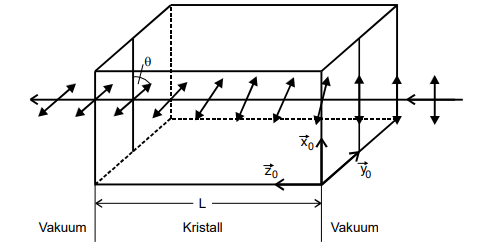
\includegraphics[scale=0.7]{fig/brechung.png}
  \caption{Darstellung von zirkularer Doppelbrechung bei Transmission eines Kristalls. \cite[1]{Anleitung}}
  \label{fig:brechung}
\end{figure}
Die Entstehung dieses Effektes beruht auf den elektrischen Dipolmomenten die im Kristall erzeugt werden können. Diese induzierten Dipole erzeugen die Polarisation $\vec{P}$ des Kristalles. Diese ist unter der Vorraussetzung eines kleinen elektrischen Feldes $\vec{E}$ proportional zu diesem. Es gilt die Beziehung:
\begin{equation}
  \vec{P}=\varepsilon_\mathrm{0} \chi \vec{E}
\end{equation}
Mit der elektrischen Feldkonstante $\varepsilon_\mathrm{0}$ und der dielektrischen Suszeptibilität $\chi$. Im Vergleich zu isotroper Materie ist die Suszeptibilität in den hier betrachteten anisotropen Kristallen eine Tensorgröße $\overline{\overline{\chi}}$. Materie ist genau dann doppeltbrechend wenn für die Suszeptibilität $\overline{\overline{\chi}}$ gilt \cite[3-5]{Anleitung}:
\begin{equation}
  \label{eqn:chitensor}
  \overline{\overline{\chi}}=\begin{pmatrix} \chi_\mathrm{xx} & \mathrm{i}\chi_\mathrm{xy} & 0 \\ -\mathrm{i}\chi_\mathrm{yx} & \chi_\mathrm{xx} & 0 \\ 0 & 0 & \chi_\mathrm{zz} \end{pmatrix}.
\end{equation}
Um die Drehung der Polarisationsebene $\vartheta$ zu bestimmen wird die Änderung $\vec{D}$ eines Feldes $\vec{E}$, das sich in Materie ausbreitet betrachet:
\begin{equation}
  \label{eqn:efeldinmaterie}
  \vec{D}=\varepsilon_0\left(1+\overline{\overline{\chi}}\right)\vec{E}.
\end{equation}
Setzt man die beiden Audrücke in (\ref{eqn:chitensor}) und (\ref{eqn:efeldinmaterie}) in die homogene Wellengleichung
\begin{equation*}
  \Box \vec{D} = 0
\end{equation*}
ein errechnet sich die Drehung $\vartheta$ \cite[3-5]{Anleitung} zu:
\begin{equation}
  \label{eqn:drehungmitchi}
  \vartheta \approx \frac{L\omega}{2c} \frac{1}{\sqrt{1+\chi_\mathrm{xx}}} \chi_\mathrm{xy}\approx \frac{L\omega}{2cn} \chi_\mathrm{xy}.
\end{equation}
Dabei ist $L$ die Länge des Kristalls, $\omega$ die Frequenz und $n$ der Brechungsindex.
\subsection{Bestimmung der effektiven Masse}
\label{sec:effektivemasse}
In diesem Abschnitt wird beschrieben wie sich mit Hilfe der Faraday-Rotation die effektive Masse bestimmen lässt. Dazu wird die Bewegungsgleichung eines gebundenen Teilchens in einem Magnetfeld $\vec{B}$ unter dem Einfluss des einfallenden Lichtstrahls und dessen elektrischen Feldes $\vec{E}$ betrachtet:
\begin{equation}
  \label{eqn:bewegung}
  m\dfrac{\partial^2\vec{r}}{\partial t^2}+K\vec{r}=-e_\mathrm{0}\vec{E}(r)-e_\mathrm{0}\dfrac{\partial \vec{r}}{\partial t}\times \vec{B}
\end{equation}
Dabei ist $\vec{r}$ die Auslenkung des Elektrons aus der Gleichgewichtslage, $K$ die Konstante, die die Bindung des Elektrons an seine Umgebung bezeichnet und $\vec{E}$ die Feldstärke des einfallenden Lichtstrahls. Nimmt man nun an, dass sowohl die Messfrequenz wesentlich höher als die Zyklotronfrequenz ist und quasifreie Ladungsträger kann der folgende Ausdruck hergeleitet werden \cite[5-8]{Anleitung}:
\begin{equation}
  \label{eqn:massewelle}
  \vartheta\approx\dfrac{e_\mathrm{0}^3}{8\pi^2\varepsilon_\mathrm{0}c^3}\dfrac{1}{m^2}\lambda^2\dfrac{NBL}{n}
\end{equation}
Damit die Gleichung \ref{eqn:massewelle} auch für die Kristallelektronen gültig bleibt setzen wir für $m$ die effektive Masse $m^*$ aus Abschnitt \ref{sec:effektive_masse} ein. Wir definieren zusätzlich die neue Größe $\vartheta_\mathrm{norm}=\dfrac{\vartheta}{L}$, die die Faraday-Rotation pro Einheitslänge in [$\SI{}{\radian\per\meter}$] angibt. Damit ergibt sich schlussendlich der folgende Ausdruck:
\begin{equation}
  \label{eqn:massewinkel}
  \vartheta_\mathrm{norm}\approx\dfrac{e_\mathrm{0}^3}{8\pi^2\varepsilon_\mathrm{0}c^3}\dfrac{1}{(m^*)^2}\lambda^2\dfrac{NB}{n}
\end{equation}
Dabei ist $e_\mathrm{0}$ die Elementarladung, $\varepsilon_\mathrm{0}$ die elektrische Feldkonstante, $c$ die Lichtgeschwindigkeit im Vakuum, $\lambda$ die Wellenlänge des einfallenden Lichtes, $N$ die Donatorenkonzentration, $B$ ist die magnetische Feldstärke, $L$ die Dicke der Probe und $n$ der Brechungsindex.
Aus dieser kann die effektive Masse der Elektronen im Kristall bestimmt werden in dem man Gleichung (\ref{eqn:massewinkel}) nach $m^*$ umstellt:
\begin{equation}
  \label{eqn:massefinal}
  m^*=\sqrt{\dfrac{e_\mathrm{0}^3}{8\pi^2\varepsilon_\mathrm{0}c^3}\dfrac{1}{\vartheta_\mathrm{frei}}\lambda^2\dfrac{NB}{n}}
\end{equation}
